% \documentclass[11pt]{article}

% \usepackage[margin=1in]{geometry}
% \usepackage{graphicx}
% \usepackage{booktabs}
% \usepackage{amsmath}
% \usepackage{hyperref}
% \usepackage{xcolor}

% \title{CS285 Milestone Report -- Offline-to-Online RL for Portfolio Optimization}
% \author{Thomas Lee}
% \date{April 2026}

% \begin{document}
% \maketitle

\documentclass[10pt]{article}
\usepackage[margin=.3in]{geometry}
\usepackage{enumitem}
\usepackage{hyperref}
\usepackage{graphicx}
\usepackage{amssymb}
\usepackage{booktabs}
\usepackage{amsmath}
\usepackage{hyperref}
\usepackage{xcolor}
\usepackage[compact]{titlesec}
\usepackage{enumitem}

\titleformat{\section}{\normalfont\Large\bfseries}{\thesection.}{0.1em}{}
\titleformat{\subsection}{\normalfont\large\bfseries}{\thesubsection.}{0.1em}{}
\titleformat{\subsubsection}{\normalfont\bfseries}{\thesubsubsection.}{0.1em}{}
\titlespacing*{\section}{0pt}{1ex}{1ex}
\titlespacing*{\subsection}{0pt}{0.5ex}{0.5ex}
\titlespacing*{\subsubsection}{0pt}{0ex}{0.5ex}

\begin{document}

\begin{center}
    \textbf{\large CS 285 Final Project Milestone Report - Thomas Lee} \\
    \textbf{Offline-to-Online (O2O) Deep Reinforcement Learning for Non-Stationary Portfolio Optimization}
\end{center}

%==============================================================
\section{Project Overview}
%==============================================================

We study \emph{offline-to-online} (O2O) deep reinforcement learning for
multi-asset portfolio allocation across the 8-asset universe
\{SPY, EEM, TLT, HYG, DBC, GLD, UUP, SHY\}.  At each rebalancing step
the agent outputs portfolio weights $w \in \Delta^{8}$ (softmax
parameterization) and receives log-return minus an $L_1$ turnover penalty
as reward.  The pipeline has three stages: (i) construct an offline
dataset from diverse behavior policies (Dirichlet, equal-weight,
momentum, risk parity); (ii) pretrain an offline RL agent on that
dataset; (iii) fine-tune online in the backtest simulator.  The current
milestone focuses on stage (ii) using Implicit Q-Learning (IQL), and in
particular on sensitivity to the core IQL knobs -- the expectile
$\tau$, the advantage temperature $\beta$, and the transaction-cost
coefficient $\lambda$.

Financial markets are a canonical non-stationary environment: the joint
distribution of asset returns shifts across volatility regimes,
interest-rate cycles, and crisis episodes.  Our training data
(2008--2020) spans two major crises -- the 2008 Global Financial Crisis
and the 2020 COVID crash -- in both of which equities fell while
bonds and gold rallied (the classic ``flight to safety'').  Offline
agents trained on this period learn to overweight duration and safe
havens during drawdowns.  However, the 2022 inflation shock broke this
40-year negative stock--bond correlation: rapid Fed rate hikes caused
\emph{both} equities and long-duration bonds to crash simultaneously.
A frozen offline policy that confidently rotates into bonds during a
drawdown will therefore fail catastrophically on the test window
(2022--2026).  This structural distribution shift is exactly the setting
where offline-to-online adaptation should help: use the cheap historical
data to learn a competent prior, then spend a small budget of online
interaction to correct the specific failure modes (here, turnover
control and regime mismatch) that offline training cannot see.

To support this investigation we have implemented a comprehensive
algorithmic suite: 12 offline RL baselines (BC, Fisher-BC, TD3+BC, AWAC,
CQL, IQL, EDAC, BCQ, MBPO, MOPO, Decision Transformer, Trajectory
Transformer), 6 online baselines via Stable-Baselines3, 5 FinRL-native
agents, 3 classical portfolio benchmarks (equal weight, inverse
volatility, Markowitz MVO), and 4 novel contributions --
\textbf{SAC-Dirichlet} (a Dirichlet policy on the probability simplex
with exact entropy), \textbf{Geodesic-CQL} (conservative Q-learning
penalized by the Fisher-Rao geodesic distance on the simplex),
a \textbf{GRU-based regime encoder} that conditions actor and critic on
a latent regime belief $h_t$, and an \textbf{O2O adaptive pipeline} that
uses KL divergence between offline and online regime distributions to
schedule the conservatism weight during fine-tuning.  All algorithms
have been smoke-tested end-to-end; the IQL ablation below is the first
full-scale experiment.

%==============================================================
\section{Experiment Description}
%==============================================================

We ran a full $3 \times 3 \times 3 = 27$ grid of IQL ablations
with the hyperparameters in Table~\ref{tab:hparams}.  All other settings
are held fixed (batch size $256$, $\gamma = 0.99$, Adam at
$3{\times}10^{-4}$, Polyak $0.005$, $20{,}000$ gradient steps, seed
$42$, offline dataset \texttt{datasets/real\_dirichlet.npz}).  Splits
are chronological: train 2008--2020, validation 2021, test 2022-Q1
through 2026-Q1.  The purpose is to characterize the \emph{sensitivity}
of an offline IQL agent under increasing market friction, and to
identify where the offline policy stops being viable without online
correction.
\vspace{-10pt}
\begin{table}[h]
\centering
\begin{tabular}{lc}
\toprule
Hyperparameter & Swept values \\
\midrule
Expectile $\tau$                  & $\{0.6,\ 0.7,\ 0.8\}$ \\
Advantage temperature $\beta$     & $\{1.0,\ 3.0,\ 10.0\}$ \\
Transaction cost $\lambda$        & $\{0,\ 0.001,\ 0.005\}$ \\
\bottomrule
\end{tabular}
\vspace{-10pt}
\caption{Ablation grid (27 runs in total).}
\label{tab:hparams}
\end{table}
\vspace{-13pt}

For every run we log a validation Sharpe curve every 1{,}000 gradient
steps and evaluate the best-validation checkpoint on the held-out test
period.  Classical baselines (equal weight, momentum, risk parity) are
computed on the same test window for reference.

%==============================================================
\section{Key Results}
%==============================================================

Aggregated results from the extracted per-run metrics (see
\texttt{figures/ablation\_summary.csv}) show a clean separation by
transaction-cost regime.  Representative values per friction level:
\vspace{-10pt}
\begin{table}[h]
\centering
\small
\begin{tabular}{lcccc}
\toprule
Regime & best val. Sharpe & test Sharpe & cum. return & max drawdown \\
\midrule
$\lambda = 0$     & $1.29$ -- $1.34$  & $0.90$ -- $0.95$   & $+0.33$ -- $+0.41$ & $0.10$ -- $0.12$ \\
$\lambda = 0.001$ & $0.59$ -- $0.64$  & $0.34$ -- $0.37$   & $+0.10$ -- $+0.11$ & $0.14$ \\
$\lambda = 0.005$ & $-2.23$ -- $-2.13$ & $-2.01$ -- $-1.95$ & $-0.47$ -- $-0.47$ & $0.47$ \\
\bottomrule
\end{tabular}
\vspace{-10pt}
\caption{Ranges across the nine $(\tau,\beta)$ cells at each transaction
cost. Values taken directly from the extracted run logs; no smoothing.}
\label{tab:by-tc}
\end{table}
\vspace{-13pt}

\begin{itemize}[noitemsep, topsep=0pt]
\item \textbf{Best configuration by validation Sharpe.}
      $\tau = 0.6,\ \beta = 3.0,\ \lambda = 0$ reaches validation Sharpe
      $1.337$ (step $10{,}000$) with test Sharpe $0.896$ and
      cumulative return $+0.413$.
\item \textbf{Best configuration by test Sharpe.}
      $\tau = 0.7,\ \beta = 1.0,\ \lambda = 0$ with test Sharpe
      $0.949$, cumulative return $+0.332$, max drawdown $0.115$.
\item \textbf{Impact of transaction costs.}  Adding even
      $\lambda = 0.001$ (10\,bps per unit turnover) halves validation
      Sharpe and roughly cuts test Sharpe to one-third.  At
      $\lambda = 0.005$ every one of the nine $(\tau,\beta)$ cells
      collapses to a \emph{strictly negative} test Sharpe of about
      $-2.0$ and a $\approx 47\%$ drawdown.
\item \textbf{Sensitivity to $\tau$ and $\beta$.}  Within a fixed
      $\lambda$, varying $\tau \in \{0.6,0.7,0.8\}$ or
      $\beta \in \{1,3,10\}$ moves validation Sharpe by at most
      $\sim 0.05$ and test Sharpe by $\sim 0.02$.  These knobs are
      effectively second-order compared to the friction coefficient.
\item \textbf{Baseline context.}  On the same test window the classical
      baselines achieve Sharpe $0.953$ (equal weight), $0.953$
      (momentum) and $1.226$ (risk parity).  The frictionless IQL
      configurations match equal weight / momentum but do not beat
      risk parity; under friction no IQL configuration is competitive.
\end{itemize}

%==============================================================
\section{Training Curves}
%==============================================================

Figure~\ref{fig:sharpe} plots validation Sharpe vs. gradient step
for 27 runs.  Figure~\ref{fig:summary} compares best-validation
Sharpe vs. test Sharpe per config.

\begin{figure}[h]
    \centering
    % First subfigure
    \begin{minipage}{0.48\textwidth}
        \centering
        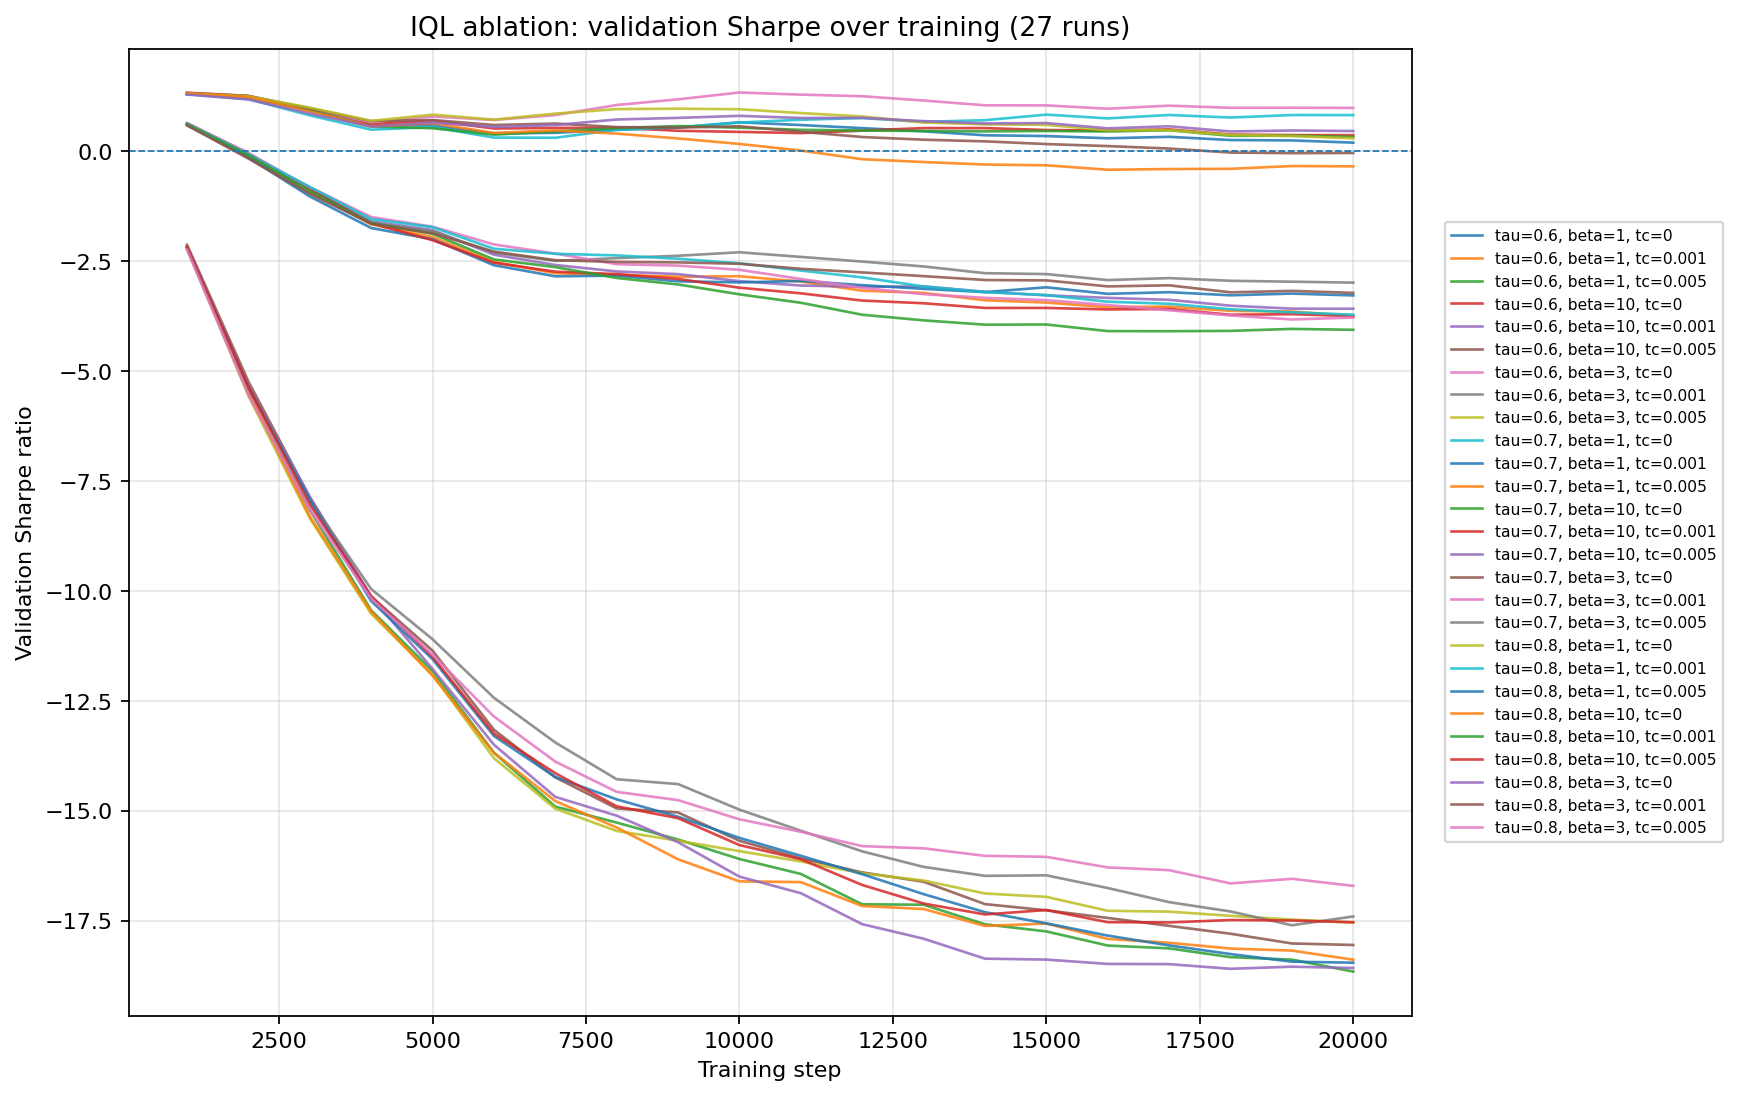
\includegraphics[width=\linewidth]{figures/iql_ablation_sharpe_curve.png}
        \caption{Validation Sharpe over training for all 27 IQL ablation runs. Three clear bands emerge, indexed by the transaction-cost coefficient $\lambda$.}
        \label{fig:sharpe}
    \end{minipage}\hfill
    % Second subfigure
    \begin{minipage}{0.48\textwidth}
        \centering
        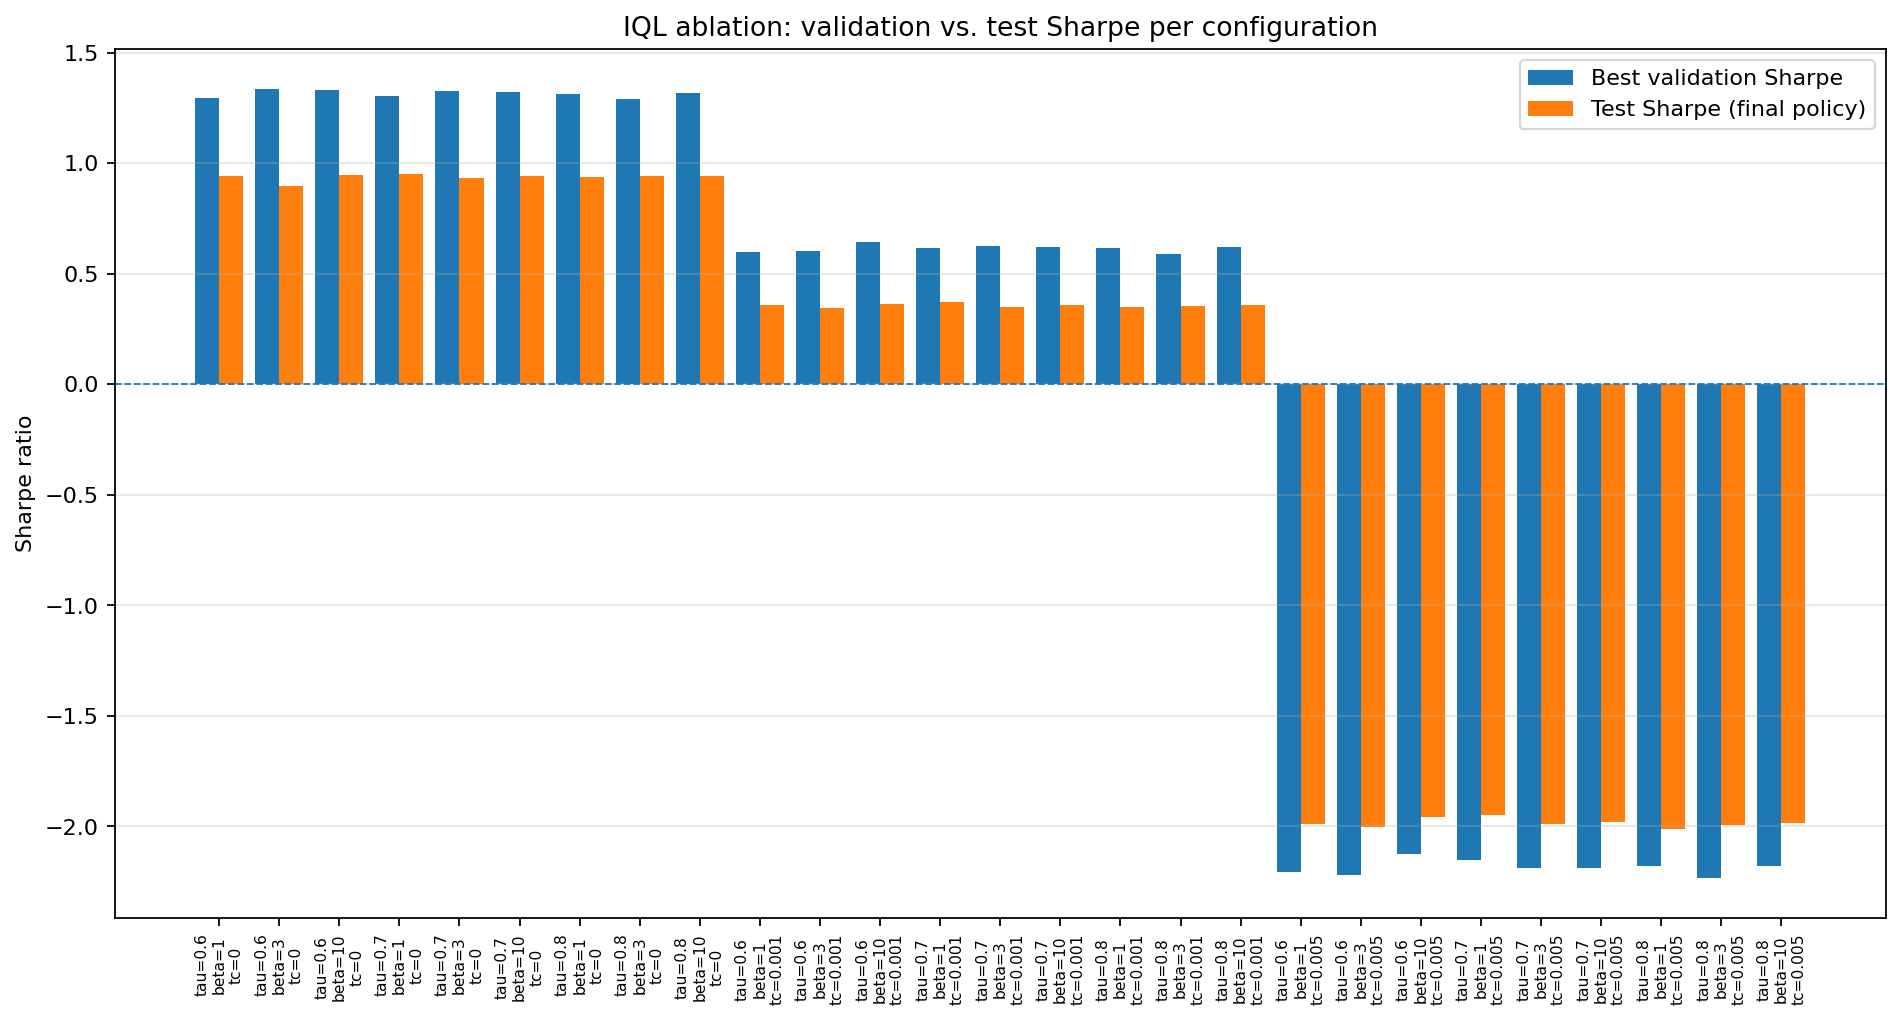
\includegraphics[width=\linewidth]{figures/iql_ablation_summary.png}
        \caption{Best-validation Sharpe vs. final test Sharpe for each $(\tau,\beta,\lambda)$ cell. The generalization gap is consistent within a friction band but the absolute level is dominated by $\lambda$.}
        \label{fig:summary}
    \end{minipage}
\end{figure}

%==============================================================
\section{Interpretation}
%==============================================================

Three observations drive the next phase of the project.

\textbf{Friction dominates.}  The dominant axis of variation in
Table~\ref{tab:by-tc} and in Figure~\ref{fig:sharpe} is $\lambda$, not
$\tau$ or $\beta$.  This is consistent with the offline dataset: the
behavior mixture (Dirichlet / equal-weight / momentum / risk parity)
induces a turnover distribution the agent cannot selectively
\emph{avoid} at training time, so as $\lambda$ grows, advantage-weighted
BC continues to imitate high-turnover actions whose \emph{realized}
reward after the penalty is now negative.

\textbf{Offline IQL is visibly unstable at moderate friction.}  The
validation Sharpe for every $\lambda > 0$ run in
Figure~\ref{fig:sharpe} peaks very early (often at the first evaluation,
step $1{,}000$) and then decays monotonically for the remainder of the
$20{,}000$ steps.  The single frictionless run that kept improving
($\tau{=}0.6,\beta{=}3.0$) peaks at step $10{,}000$.  Early stopping is
therefore doing a lot of the work in this sweep, which is itself a
symptom of offline distribution shift rather than a robust training
signal.

\textbf{Motivation for O2O.}  The agent is not catastrophically bad at
$\lambda = 0$ -- it matches the equal-weight benchmark -- but it
collapses the moment we introduce realistic execution cost.  Because
turnover is the direct lever of transaction cost, correcting this from
logged data alone is hard: the behavior mix does not contain enough
low-turnover, high-Sharpe counterfactuals to re-weight.  A small amount
of online interaction specifically targeting turnover feedback is the
natural next step, which is exactly the setting O2O is designed for.

%==============================================================
\section{Future Work}
%==============================================================

\begin{itemize}[noitemsep, topsep=0pt]
\item \textbf{Offline RL improvements.}
      Run the remaining 11 offline baselines (BC, Fisher-BC, TD3+BC,
      AWAC, CQL, EDAC, BCQ, MBPO, MOPO, Decision Transformer,
      Trajectory Transformer) on the same chronological split to
      determine whether IQL's friction sensitivity is algorithm-specific
      or a shared failure mode of offline methods.  Test multi-step
      returns ($n \in \{1, 3, 5\}$) via the implemented
      \texttt{NStepReplayBuffer} to see whether longer credit
      assignment horizons help under transaction costs.

\item \textbf{Online fine-tuning strategy.}
      Deploy the O2O adaptive pipeline: Geodesic-CQL pre-trains offline
      on 2008--2020, then SAC-Dirichlet fine-tunes online on the
      2022--2026 test window.  The KL divergence between offline and
      online regime encoder hidden states adaptively scales the CQL
      conservatism weight $\beta_t = \sigma(\lambda \cdot
      \mathrm{KL}(h_{\text{offline}} \| h_{\text{online}}))$, allowing
      the agent to shed conservatism only when the current regime
      resembles the training distribution.  We will compare the full O2O
      pipeline against (a) frozen offline policy, (b) online-only
      SAC-Dirichlet, and (c) naive fine-tuning without adaptive CQL
      scheduling.

\item \textbf{Environment improvements.}
      Integrate FRED macroeconomic features (10-year yield, Fed Funds
      rate, CPI, unemployment, NFCI) and SF~Fed Daily News Sentiment
      Index as additional observation channels.  These should provide
      leading indicators of regime shifts that pure price-based features
      miss.  Test via modality ablation: price only $\to$ +macro $\to$
      +sentiment $\to$ +Alpaca news embeddings (384-d).

\item \textbf{Model improvements.}
      Compare SAC-Dirichlet (exact simplex entropy) against
      Gaussian-softmax SAC and PPO variants (MLP, LSTM, Transformer) as
      the online fine-tuning backbone.  Evaluate Geodesic-CQL
      (Fisher-Rao distance penalty) against vanilla CQL
      ($\mathbb{E}_\pi[Q] - \mathbb{E}_{\mathcal{D}}[Q]$) to isolate the
      contribution of geometry-aware conservatism.  Sweep the CQL penalty
      strength $\alpha \in \{1, 3, 5, 10\}$ on the validation split.

\item \textbf{O2O extension experiments.}
      Implement a Bayesian regime encoder that outputs a posterior
      distribution $q(h_t | o_{t-k:t}) = \mathcal{N}(\mu_t, \sigma_t^2)$
      over the latent regime state, enabling (a)~uncertainty-weighted CQL
      penalties $\beta_t \propto \sigma(\lambda \cdot \mathrm{KL} +
      \gamma \cdot \mathrm{Var}[h_t])$ that maintain conservatism under
      epistemic uncertainty, and (b)~Thompson-sampling exploration where
      high regime uncertainty naturally drives diverse behavior.  Run the
      full Bayesian O2O pipeline on both the ETF universe (2008--2026)
      and the mutual-fund proxy universe (1995--2026, capturing the
      Dot-Com bubble) across 3 seeds for statistical confidence.
\end{itemize}

% %==============================================================
% \section{Project Positioning}
% %==============================================================

% Financial markets are a canonical non-stationary RL environment:
% return distributions, volatility regimes, and cross-asset correlations
% drift on horizons shorter than any practical training window.  Offline
% data is abundant -- decades of daily bars are cheap -- but biased:
% historical trajectories reflect a specific sequence of regimes and a
% specific behavior mix, so a purely offline policy inherits whatever
% blind spots that mix has (here, uncontrolled turnover).  Online
% interaction, conversely, is expensive and risky: every exploratory
% trade is a real loss, which tightly caps the sample budget.
% Offline-to-online RL is the natural framing for this tension: use
% cheap historical data to learn a competent prior, then spend a small,
% carefully-budgeted amount of online interaction to correct the
% failure modes that offline training cannot see.  The ablation
% presented here isolates exactly such a failure mode -- turnover under
% friction -- and motivates the O2O component of the final project.

\end{document}
